\section{Aufgaben}

\subsection{Magnetfeld eines Kreiszylinders mit Bohrung}

a) Betrachten Sie zunächst einen in der Länge unendlich ausgedehnten zylinderförmigen Leiter
mit Radius $R$ , der von einem Strom konstanter Stromdichte $\vec{j}$ durchflossen wird. Berechnen
Sie mithilfe des Satzes von Stokes das Magnetfeld sowohl innerhalb als auch außerhalb des
Leiters.

\noindent b) Nehmen Sie nun an, dass sich im Zylinder aus Teil a) eine Bohrung parallel zur Symmetrieachse des Leiters im Abstand a von der Achse bendet. Die Bohrung hat den Radius $R_0$ und es gilt $a + R_0 < R$ (s. Abbildung). Berechnen Sie das Feld im Inneren der Bohrung. Gehen Sie dabei folgendermaßen vor:
Betrachten Sie die Konguration aus der Aufgabenstellung als Superposition eines stromdurchossenen Vollzylinders wie in Teil a) einerseits und eines Zylinders an der Stelle der Bohrung andererseits, der von einem Strom konstanter Stromdichte $− \vec{j}$ durchflossen wird.
Berechnen Sie dann das Feld im Inneren der Bohrung als Superposition der Felder dieser beiden Zylinder.

\noindent c) Betrachten Sie nun ein bewegtes Punktteilchen der Masse $m$ und der Ladung $q$, das sich
innerhalb der Bohrung befindet (in der wir ein Vakuum annehmen). Beschreiben Sie qualitativ, wie mögliche stabile Bahnen aussehen. Berechnen Sie, welche Geschwindigkeit das Punktteilchen maximal haben darf, damit es die Wände der Bohrung nicht berührt.


\subsection{Schwingender Dipol}

Betrachten Sie eine kreisförmige Leiterschleife mit Radius $R$, die sich in der $xy$-Ebene befindet und von einem Strom $I$ durchflossen wird. Im Mittelpunkt der Leiterschleife befindet sich ein kleiner magnetischer Dipol, z.B. der Spin eines Elektrons, der in Richtung des B-Feldes ausgerichtet ist und der sich nur in z-Richtung bewegen kann.

\noindent a) Geben Sie den allgemeinen Ausdruck der potentiellen Energie $E_{pot}$ des Dipols als Funktion seiner Auslenkung $z$ an.

\noindent b) Entwickeln Sie $E_{pot}$ bis in zweite Ordnung in $z$.

\noindent c) Bestimmen Sie die Schwingungsfrequenz $\omega$, mit der der Dipol bei kleinen Auslenkungen um $z = 0$ herum schwingt.
\newpage
\subsection{Netzwerke}

Der südamerikanische Zitteraal (Electrophorus electricus) setzt Stromstöße ein, um Beutetiere zu lähmen und um sich und sein Revier zu verteidigen. Er verfügt über ein Netzwerk von Spannungsquellen, von denen ca. 5000 zu je 0,15 V mit einem Innenwiderstand von 0,25 Ω in Reihe geschaltet sind. Etwa 140 solcher Reihen sind parallel geschaltet und entlang des Körpers des Tiers angeordnet.

\noindent (a) Wie groß ist die Spannung und der Innenwiderstand zwischen den Enden des Zitteraals?

\noindent (b) Wie groß ist der elektrische Strom durch das Wasser in der Umgebung des Zitteraals unter der Annahme eines elektrischen Widerstands von 800 Ω?

\noindent (c) Wie groß ist der elektrische Strom, wenn man eine Spannung von 12 V an gegenüberliegende Ecken anschließt?


\begin{figure}
 \centering
 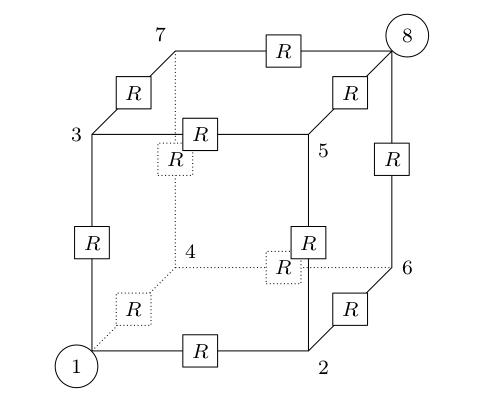
\includegraphics[width= 8cm, height= 8cm]{media/screen.png}
\end{figure}
